\chapter{Tensor-RNN: bridge between tensor networks and neural networks}
\label{ch:tensor-rnn}

Comparing tensor network (TN) quantum states in \cref{ch:tn} and neural quantum states (NQSs) in \cref{sec:nqs}, we can see that TNs have deeper background in physics, as their representations of the ground states of some important physical systems are found by construction, and their analytical properties such as the entanglement entropy and the spatial correlations are proven. They are also more controllable, in the sense that we can systematically improve the accuracy of variational approximation by increasing their bond dimensions. Their relatively simple multilinear architectures are suitable for second-order optimizations, which have better convergence properties towards the ground state than the first-order optimizations usually used for neural networks. However, the 1D matrix product state (MPS) is not expressive enough for 2D and higher-dimensional systems, and the 2D projected entangled-pair state (PEPS) cannot be efficiently contracted.

On the contrary, NQSs are proven to have the expressiveness of universal approximation, and they are practically successful in representing complicated ground states, such as spin liquids, with high accuracy and efficiency. However, their interpretability and controllability are worse than TNs. Their analytical properties, the relation between the accuracy of variational approximation and their hyperparameters, such as the numbers of layers and channels, as well as the optimization methods to fully exploit their expressiveness, are all under research.

Since the initial proposal of NQSs, there has been continuing research on their ability to represent certain classes of quantum states~\cite{gao2017efficient, carleo2018constructing, sharir2022neural}. Exact mappings have been constructed between TNs and NQSs, especially restricted Boltzmann machines (RBMs)~\cite{glasser2018neural, chen2018equivalence} with relatively simple architectures in NQSs. Meanwhile, the mapping from TNs to recurrent neural networks (RNNs) has been studied from the viewpoint of recurrent arithmetic circuits~\cite{levine2017long, levine2019quantum}, which suggests that the extra expressiveness of RNNs over TNs can be attributed to their reuse of information between sites. There have also been attempts to incorporate the multilinear contractions of TNs into NQSs in various ways, which can produce greater expressiveness than the usual linear layers~\cite{hibat2021variational, hibat2022supplementing, chen2023antn}.

In the following, we present a series of NQS architectures, namely MPS-RNN and tensor-RNN~\cite{wu2023tensor}, which combine the strengths of TNs and RNNs. They can achieve higher numerical accuracy than MPS and PEPS on 2D systems, show the desired analytical properties of entanglement entropy and spatial correlations, and get systematically improved by increasing the bond dimension, which is the only hyperparameter for their architectures. Moreover, they support exact sampling and efficient evaluation, which lead to the reduction of practical computation time compared to PEPS.

\section{Vanilla MPS-RNN}

We start from the aforementioned definition of an MPS with bond dimension $\chi$, on $N$ sites of spin-$\frac{1}{2}$ particles:
\begin{equation}
\psi(\vs) = \sum_{a_0, \ldots, a_N = 1}^\chi \prod_{i = 1}^N M^{(i)}_{s_i; a_i, a_{i - 1}}.
\tag{\ref{eq:mps}}
\end{equation}
Note that we use $1$-based indexing for the spatial and the bond dimensions, which is consistent with the notations in previous chapters, as opposed to the $0$-based indexing in Ref.~\cite{wu2023tensor}, which can be more convenient for software implementation. The many-body probability $q(\vs) = |\psi(\vs)|^2$ can be factorized into autoregressive (AR) conditional probabilities~\cite{ferris2012perfect, han2018unsupervised, wei2022sequential}:
\begin{equation}
q(\vs) = \prod_{i = 1}^N q_i(s_i \mid \vs_{< i}),
\tag{\ref{eq:autoreg}}
\end{equation}
which are suitable for exact sampling. Each conditional probability is formally written as
\begin{align}
q_i(s_i \mid \vs_{< i}) &=
\frac{\tilde{q}_i(s_i \mid \vs_{< i})}{\sum_s \tilde{q}_i(s \mid \vs_{< i})}, \\
\tilde{q}_i(s_i \mid \vs_{< i}) &=
\vh^{(i) \dagger}(s_i, \vs_{< i})\,\mga^{(i)} \vh^{(i)}(s_i, \vs_{< i}), \label{eq:mps-cond-prob} \\
h^{(i)}_{a_i}(\vs_{\le i}) &=
\sum_{a_1, \ldots, a_{i - 1}}
\prod_{j = 1}^i M^{(j)}_{s_j; a_j, a_{j - 1}}, \\
\gamma^{(i)}_{b_i, a_i} &=
\sum_{\substack{a_{i + 1}, \ldots, a_V \\ b_{i + 1}, \ldots, b_V \\ s_{i + 1}, \ldots, s_V}}
\prod_{j = i + 1}^V M^{(j) *}_{s_j; b_j, b_{j - 1}} M^{(j)}_{s_j; a_j, a_{j - 1}}, \label{eq:mps-gamma}
\end{align}
where $\vh^{(i)}$ is a vector of size $\chi$, denoting the partially contracted sites up to the site $i$, and depending on the spins $\vs_{\le i}$, while $\mga^{(i)}$ is a $\chi \times \chi$ matrix, denoting the partially contracted sites and their conjugates after the site $i$.

\begin{figure}[htb]
\centering
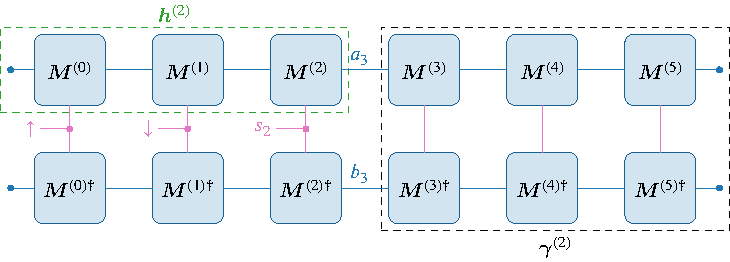
\includegraphics[width=0.8\linewidth]{ch9/mps_cond_prob.pdf}
\caption[Tensor diagram for conditional probability in MPS]{
Tensor diagram for the unnormalized conditional probability $\tilde{q}_3(s_3 \mid s_1 = \spinup, s_2 = \spindown)$ as in \cref{eq:mps-cond-prob}. An MPS with six sites is shown as an example.
This figure is reproduced from Fig.~S1 in the supplemental material for Ref.~\cite{wu2023tensor}.
}
\label{fig:mps-cond-prob}
\end{figure}

The tensor diagram for the unnormalized conditional probability in \cref{eq:mps-cond-prob} is shown in \cref{fig:mps-cond-prob}. Note that the solid dot with $r$ indices denotes the rank-$r$ Kronecker tensor
\begin{equation}
\delta_{i_1, \ldots, i_r} = \begin{cases}
1, & i_1 = \cdots = i_r \\
0, & \text{otherwise}
\end{cases},
\end{equation}
and when $r = 1$ it simply sums over the index. As edge cases, we have
\begin{equation}
h^{(0)}_a = 1 \quad \forall a,
\end{equation}
which is just the top leftmost solid dot, and
\begin{equation}
\gamma^{(N)}_{b, a} = 1 \quad \forall a, b,
\end{equation}
which is the direct product of the rightmost two solid dots.

The MPS can be optimized using VMC with AR sampling. At the beginning of each optimization step of VMC, we precompute $\mga^{(N - 1)}, \ldots, \mga^{(1)}$ sequentially during a usual contraction of $\ip{\psi}$, which are independent of the input spins. Then in each AR sampling step $i$, we update $\vh^{(i)}$ by
\begin{equation}
\vh^{(i)}(s_i) = \mM^{(i)}_{s_i} \vh^{(i - 1)},
\label{eq:mps-rnn-h}
\end{equation}
which can be interpreted as updating the hidden memory in an RNN as in \cref{eq:rnn-update}. Note that the spin $s_i$ is a free variable at this point, while all previous spins $\vs_{< i}$ that are input to $\vh^{(i)}$ are already determined. Also, unlike the conventional RNN, in the MPS we do not share parameters $\mM^{(i)}$ between different sites $i$. After obtaining $\vh^{(i)}$, we compute the unnormalized conditional probability
\begin{equation}
\tilde{q}_i(s_i \mid \vs_{< i}) = \vh^{(i) \dagger}(s_i)\,\mga^{(i)} \vh^{(i)}(s_i),
\label{eq:mps-rnn-q}
\end{equation}
and normalize it if needed, which can be interpreted as the output layer of the RNN as in \cref{eq:rnn-output}. The tensor diagrams for this AR sampling step are shown in \cref{fig:mps-h-p}.

\begin{figure}[htb]
\centering
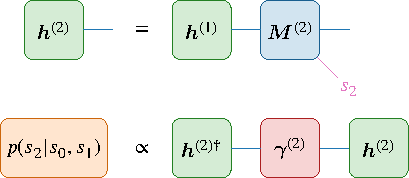
\includegraphics[width=0.5\linewidth]{ch9/mps_h_p.pdf}
\caption[Tensor diagrams for an AR sampling step of MPS]{
Tensor diagrams for updating the memory $\vh^{(i)}$ as in \cref{eq:mps-rnn-h}, and computing the conditional probability $q_i(s_i \mid \vs_{< i})$ as in \cref{eq:mps-rnn-q}, in an AR sampling step of MPS.
This figure is reproduced from Fig.~1~(b) in Ref.~\cite{wu2023tensor}.
}
\label{fig:mps-h-p}
\end{figure}

Therefore, the MPS is exactly mapped to an RNN architecture with memory size $\chi$, linear updates of the memory in \cref{eq:mps-rnn-h}, and a bilinear output layer in \cref{eq:mps-rnn-q}. To avoid precomputing $\{\mga^{(i)}\}$ from $\{\mM^{(i)}\}$, and make a generalization from the MPS, we treat $\{\mga^{(i)}\}$ as variational parameters besides $\{\mM^{(i)}\}$, where each $\{\mM^{(i)}\}$ and $\{\mga^{(i)}\}$ is independent of each other. Therefore, the RNN architecture has greater expressiveness than the MPS, but not every trained RNN can be mapped back to an MPS. In the following, we refer to this architecture as the vanilla MPS-RNN.

Besides the probability $q(\vs)$, the complete definition of the wave function also includes the phase $\phi(\vs)$:
\begin{equation}
\psi(\vs) = \sqrt{q(\vs)} \rme^{\rmi \phi(\vs)}.
\tag{\ref{eq:psi-q-phi}}
\end{equation}
After the AR sampling of the vanilla MPS-RNN, $\phi(\vs)$ is obtained by
\begin{equation}
\phi(\vs) = \arg \sum_{a} h^{(N)}_a.
\label{eq:mps-rnn-phase}
\end{equation}
The computational graph for the vanilla MPS-RNN to evaluate $\psi(\vs)$ is shown in \cref{fig:rnn-psi}.

\begin{figure}[htb]
\centering
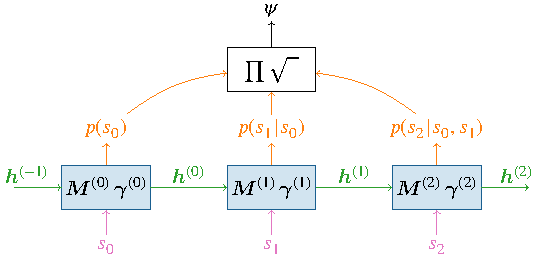
\includegraphics[width=0.7\linewidth]{ch9/rnn_psi.pdf}
\caption[Computational graph for vanilla MPS-RNN]{
Computational graph for the vanilla MPS-RNN to evaluate the wave function $\psi(\vs)$, where three sites are shown as an example.
Every site $i$ has the variational parameters $\mM^{(i)}$ and $\mga^{(i)}$, takes the spin $s_i$ and the previous memory $\vh^{(i - 1)}$ as inputs, and outputs the conditional probability $q(s_i \mid \vs_{< i})$ and the updated memory $\vh^{(i)}$.
The phase part is omitted for simplicity.
This figure is reproduced from Fig.~1~(a) in Ref.~\cite{wu2023tensor}.
}
\label{fig:rnn-psi}
\end{figure}

The vanilla MPS-RNN takes $O(N \chi^2)$ time and space to sample the configuration $\vs$ and evaluate the wave function $\psi(\vs)$. It is worth noting that MPS can exactly represent the ground states of 1D gapped systems, and every MPS can be exactly mapped to a vanilla MPS-RNN, so the nonlinear activation functions in the update rules of conventional RNNs are unnecessary to represent these states.

\section{1D MPS-RNN}

We make a few modifications to the vanilla MPS-RNN to reduce its computation time and improve its training stability, while also slightly increase its expressiveness. Each matrix $\mga^{(i)}$ in \cref{eq:mps-gamma} is positive semidefinite, so we diagonalize it by
\begin{equation}
\mga^{(i)} = \mU^{(i)} \diag\left( \vet^{(i)} \right) \mU^{(i) \dagger},
\end{equation}
where $\mU^{(i)}$ is a unitary matrix, and $\vet^{(i)}$ is a real and positive vector, which is further parameterized by the real vector $\ln \vet^{(i)}$. In the following, we absorb $\mU^{(i)}$ into the definition of $\mM^{(i)}$, and also the resulting $\vh^{(i)}$:
\begin{align}
\mM^{(i)} &\gets \mU^{(i)} \mM^{(i)} \mU^{(i - 1) \dagger}, \\
\vh^{(i)} &\gets \mU^{(i)} \vh^{(i)}.
\end{align}
Therefore, the probability in \cref{eq:mps-cond-prob} is simplified to
\begin{equation}
\tilde{q}_i(s_i \mid \vs_{< i}) = \sum_s \eta^{(i)}_s \left| h^{(i)}_s \right|^2,
\label{eq:mps-rnn-p-eta}
\end{equation}
where the number of parameters and the computation time are reduced without loss of expressiveness.

Then we generalize the update rule \cref{eq:mps-rnn-h} by adding a term $\vv^{(i)}$, which is a vector of size $\chi$ and depends on the spin $s_i$, i.e., it is a $2 \times \chi$ tensor when we view $s_i$ as a free variable. Then the update rule becomes
\begin{equation}
\tilde{\vh}^{(i)}(s_i) = \mM^{(i)}_{s_i} \vh^{(i - 1)} + \vv^{(i)}_{s_i}.
\label{eq:mps-rnn-h-v}
\end{equation}
The expressiveness of the architecture with the term $\vv^{(i)}$ and with bond dimension $\chi$ is not greater than that without the term $\vv^{(i)}$ and with bond dimension $\chi + 1$, because $\vv^{(i)}$ can be absorbed into $\mM^{(i)}$ as an extra row. Moreover, we normalize the intermediate result after each AR sampling step:
\begin{equation}
\vh^{(i)}(s_i) = \frac
{\tilde{\vh}^{(i)}(s_i)}
{\sqrt{\sum_s \tilde{\vh}^{(i) \dagger}(s) \tilde{\vh}^{(i)}(s)}},
\end{equation}
which acts similarly to the sigmoid function in conventional RNN architectures to bound the intermediate result and avoid gradient explosion~\cite{pascanu2013difficulty}. When analyzing a trained ansatz, we can always absorb the normalization into $\mM^{(i)}$.

We also generalize the phase in \cref{eq:mps-rnn-phase} to a sum of ``local phases'':
\begin{align}
\phi(\vs) &= \sum_i \phi^{(i)}(\vs_{\le i}), \label{eq:mps-rnn-phase-sum} \\
\phi^{(i)}(\vs_{\le i}) &= \arg\left( \vw^{(i) \transpose}_{s_i} \vh^{(i)}(\vs_{\le i}) + c^{(i)}_{s_i} \right), \label{eq:mps-rnn-phase-local}
\end{align}
where each local phase $\phi^{(i)}(\vs_{\le i})$ is obtained from a linear transformation of the memory $\vh^{(i)}(\vs_{\le i})$, whose parameters $\vw^{(i)}$ and $c^{(i)}$ depend on the spin $s_i$. Therefore, the gradient information from every site, rather than only the last site, can more directly affect the phase during training. It is worth noting that the phasor sum in \cref{eq:phasor-sum} can be an alternative to the simple sum in \cref{eq:mps-rnn-phase-sum}.

The RNN architecture defined by the update rule in \cref{eq:mps-rnn-h-v}, the output layer in \cref{eq:mps-rnn-p-eta}, and the phase in \cref{eq:mps-rnn-phase-local} is named 1D MPS-RNN, which is more suitable for practical computations than the vanilla one, in terms of the computation time and the numerical stability in training.

\section{2D MPS-RNN}
\label{sec:2d-mps-rnn}

Next, we investigate the generalization of the MPS-RNN to 2D lattices, which should ideally capture the area law of entanglement entropy and the algebraically decaying correlations in the 2D systems of interest, while still support efficient evaluation in polynomial time and space, as well as AR sampling. An intuitive attempt is to include the memories from two previous neighboring sites as inputs for the update rule in \cref{eq:mps-rnn-h-v}:
\begin{equation}
\tilde{\vh}^{(x, y)}(s_{x, y}) =
\mM^{(x, y)}_{\text{y}; s_{x, y}} \vh^{(x, y - 1)}
+ \mM^{(x, y)}_{\text{x}; s_{x, y}} \vh^{(x - 1, y)}
+ \vv^{(x, y)}_{s_{x, y}},
\label{eq:mps-rnn-h-2d}
\end{equation}
where we use the 2D indexing $(x, y)$ instead of the 1D indexing $i$ for the sites. In all the reported results we use the snake order as in \cref{fig:mps-order}~(b), and for simplicity we assume $y$ is odd in \cref{eq:mps-rnn-h-2d}, so $x$ increases in the snake order. On each site, there are two matrices $\mM^{(x, y)}_\text{x}$ and $\mM^{(x, y)}_\text{y}$ to transform the two input memory vectors. The tensor diagram for this update rule is shown in \cref{fig:mps-rnn-h-2d}. The RNN architecture defined by \cref{eq:mps-rnn-h-2d} as well as the previous \cref{eq:mps-rnn-p-eta,eq:mps-rnn-phase-local} is named 2D MPS-RNN, and its computational graph to evaluate the wave function is shown in \cref{fig:tensor-rnn-all}.

\begin{figure}[htb]
\centering
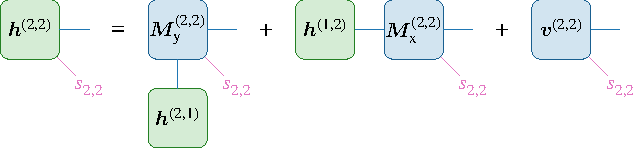
\includegraphics[width=0.7\linewidth]{ch9/mps_rnn_2d_h.pdf}
\caption[Tensor diagram for memory update of 2D MPS-RNN]{
Tensor diagram for updating the memory $\vh^{(2, 2)}$ of the 2D MPS-RNN as in \cref{eq:mps-rnn-h-2d}.
The memories from the two previous neighboring sites $\vh^{(1, 2)}$ and $\vh^{(2, 1)}$ are taken as inputs.
}
\label{fig:mps-rnn-h-2d}
\end{figure}

With the added vertical connections, the time and the space complexities to sample the configuration $\vs$ and evaluate the wave function $\psi(\vs)$ do not change asymptotically compared to the 1D case. The 2D MPS-RNN is more suitable for capturing the isotropic correlations in 2D systems, because the correlations between vertically neighboring sites no longer need to propagate $O(L)$ steps with exponential decay, which we will show in \cref{sec:tensor-rnn-corr}.

However, the 2D MPS-RNN does not have exponentially greater expressiveness than the 1D MPS-RNN to asymptotically produce the area law of entanglement entropy. It is proven that every 2D MPS-RNN with bond dimension $\chi$ can be exactly represented by a 1D MPS-RNN with bond dimension $L \chi$, because each memory $\vh^{(x, y)}$ is a linear combination of the memories $\left\{ \vh^{(x, y - 1)} \mid 1 \le x \le L\,\right\}$ in the previous row.

\begin{figure}[htb]
\centering
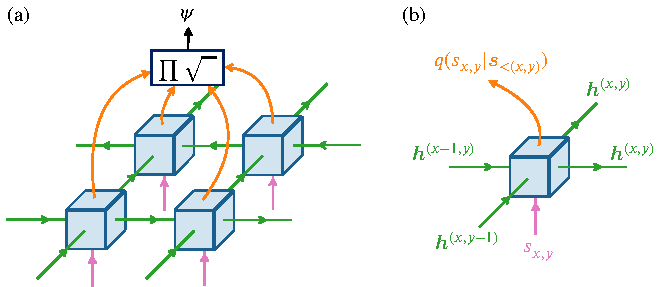
\includegraphics[width=0.7\linewidth]{ch9/tensor_rnn_all.pdf}
\caption[Computational graph for 2D MPS-RNN]{
Computational graph for the 2D MPS-RNN to evaluate the wave function $\psi(\vs)$.
In (a), four sites arranged in the snake order are shown as an example, and the phase part is omitted for simplicity.
In (b), we focus on one site at $(x, y)$, assuming $x$ increases in the snake order.
The site has the variational parameters $\mM^{(x, y)}_\text{x}$, $\mM^{(x, y)}_\text{y}$, and $\vet^{(x, y)}$, takes the spin $s_{x, y}$ and the memories $\vh^{(x - 1, y)}$ and $\vh^{(x, y - 1)}$ as inputs, and outputs the conditional probability $q(s_{x, y} \mid \vs_{< (x, y)})$ and the updated memory $\vh^{(x, y)}$.
The updated memory will be used in two future neighboring sites.
This figure is reproduced from Fig.~2 in Ref.~\cite{wu2023tensor}.
}
\label{fig:tensor-rnn-all}
\end{figure}

\section{Tensor-RNN}
\label{sec:tensor-rnn}

We continue to seek for other update rules that are expressive enough to produce the area law. Inspired by the higher-rank tensors in PEPS, we add a tensor term to the update rule in \cref{eq:mps-rnn-h-2d}, then it can be written in components as
\begin{align}
\tilde{h}^{(x, y)}_a(s_{x, y}) = &\phantom{{}+{}} \sum_{b, c} T^{(x, y)}_{s_{x, y}; a, b, c} h^{(x - 1, y)}_b h^{(x, y - 1)}_c \nonumber \\
&+ \sum_b M^{(x, y)}_{\text{y}; s_{x, y}; a, b} h^{(x, y - 1)}_b
+ \sum_b M^{(x, y)}_{\text{x}; s_{x, y}; a, b} h^{(x - 1, y)}_b \nonumber \\
&+ v^{(x, y)}_{s_{x, y}; b}\,,
\label{eq:tensor-rnn-h}
\end{align}
where $\mT^{(x, y)}$ is a $\chi \times \chi \times \chi$ tensor and depends on the spin $s_{x, y}$, and the tensor diagram for this update rule is shown in \cref{fig:tensor-rnn-h}. The RNN architecture defined by \cref{eq:tensor-rnn-h} as well as the previous \cref{eq:mps-rnn-p-eta,eq:mps-rnn-phase-local} is named tensor-RNN. Its computational graph is the same as \cref{fig:tensor-rnn-all}, except that there are the additional variational parameters $\mT^{(x, y)}$ on each site $(x, y)$.

\begin{figure}[htb]
\centering
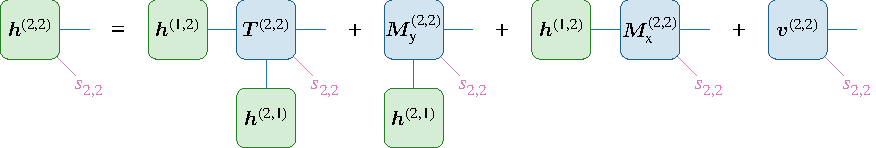
\includegraphics[width=\linewidth]{ch9/tensor_rnn_h.pdf}
\caption[Tensor diagram for memory update of tensor-RNN]{
Tensor diagram for updating the memory $\vh^{(2, 2)}$ of the tensor-RNN as in \cref{eq:tensor-rnn-h}.
This figure is reproduced from Fig.~3 in Ref.~\cite{wu2023tensor}.
}
\label{fig:tensor-rnn-h}
\end{figure}

The tensor-RNN takes $O(N \chi^3)$ time and space to sample the configuration $\vs$ and evaluate the wave function $\psi(\vs)$, which avoids the exponential computational complexity of PEPS. It can actually produce the area law, as proven by construction in Section~S5 of the supplemental material for Ref.~\cite{wu2023tensor}. This is also supported by numerical evidence in systems more common than that artificial construction, which we will show in \cref{sec:tensor-rnn-magnitude}.

When the $O(\chi^3)$ time and space complexities introduced by the tensor term $\mT$ are undesired for large systems, we can further parameterize it by
\begin{equation}
T_{a, b, c} = \sum_{a', b', c' = 1}^{\chi'} K_{a', b', c'} U_{\text{o}; a, a'}  U_{\text{x}; b, b'} U_{\text{y}; c, c'},
\label{eq:tensor-decomp}
\end{equation}
which is known as the Tucker decomposition~\cite{tucker1966some}, where $\mK$ is a smaller ``kernel'' tensor of size $\chi' \times \chi' \times \chi'$, $\mU_\text{x}$, $\mU_\text{y}$, and $\mU_\text{o}$ are $\chi \times \chi'$ matrices to transform the $x$-directional input, the $y$-directional input, and the output respectively, and we omit the spatial and the spin indices for clarity. The parameter $\chi'$ controls the balance between the expressiveness and the computational cost of the decomposed tensors, and in the reported results we choose $\chi' = \chi^\frac{2}{3}$, rounded up to an integer, so the time and the space complexities to contract $\mT$ are kept to $O(\chi^2)$. The resulting architecture is referred to as the compressed tensor-RNN.

\section{Hierarchical initialization}

The ansatzes we have introduced form a hierarchy: MPS $\subsetneq$ 1D MPS-RNN $\subsetneq$ 2D MPS-RNN $\subsetneq$ compressed tensor-RNN $\subsetneq$ tensor-RNN, where each architecture can exactly represent any architecture to its left with the same bond dimension. This property can be utilized in the training of the ansatzes. We first optimize an MPS using DMRG, then convert it to a 1D MPS-RNN, which represents the same wave function but has more potential expressiveness, and continue to train all its parameters. When the 1D MPS-RNN is sufficiently trained, we convert it to a 2D MPS-RNN and repeat the procedure, until we obtain the tensor-RNN.

This procedure is referred to as the hierarchical initialization. It provides the initial parameters at reasonably low energies for each ansatz, and prevents them from getting stuck in local minima and saddle points with high energies. For non-stoquastic Hamiltonians, it also provides reasonable sign structures from DMRG, which can be hard to obtain by gradient-based optimizers, as discussed in \cref{sec:amp-phase}. This procedure is a particular advantage from our approach of exact mappings, which cannot be performed in other hybrid architectures of TN and RNN~\cite{hibat2021variational, hibat2022supplementing, chen2023antn}.

\section{Numerical results}

\subsection{Variational energy}

The performances of the above ansatzes are demonstrated in numerical experiments using the antiferromagnetic Heisenberg model (AFHM) and the transverse-field Ising model (TFIM) on 2D square and triangular lattices with open boundary conditions (OBC), as defined in \cref{sec:qu-sys}.

We first investigate the variational energy as a function of the bond dimension which is the only hyperparameter in the architectures of these ansatzes and controls their overall sizes, as shown in \cref{fig:tensor-rnn-energy-chi}. We can clearly see that the 2D ansatzes reach the same error as the 1D ones with bond dimensions less by one to two orders of magnitude, which is attributed to the vertical connections. Moreover, the error can be systematically reduced as the bond dimension increases. For the tensor-RNN, the reduction of the error particularly exhibits a power law, which can be fitted by a straight line on the log-log plot, and on the square lattice it eventually outperforms the best result of PEPS~\cite{liu2017gradient} to the author's knowledge.

\begin{figure}[htb]
\centering
\hspace*{-0.05\linewidth}
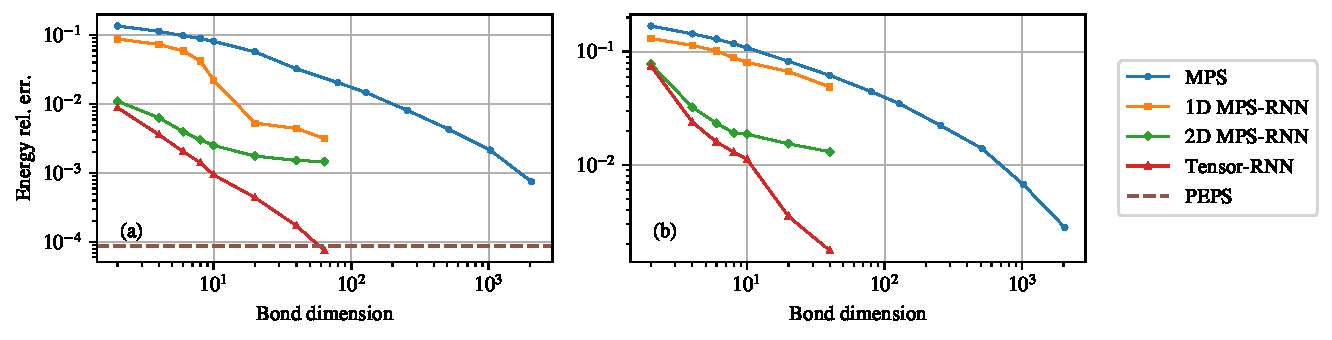
\includegraphics[width=1.1\linewidth]{ch9/tensor_rnn_energy_chi.pdf}
\caption[Variational energy vs. bond dimension for tensor-RNN]{
Variational energy as a function of the bond dimension $\chi$, for the AFHM on (a) square and (b) triangular lattice with $10 \times 10$ sites and open boundary conditions (OBC). The comparison is made between MPS (optimized by DMRG) and the ansatzes in this chapter (optimized by VMC with hierarchical initialization). The results are shown as the relative error from (a) QMC~\cite{sandvik1997finite} and (b) DMRG with $\chi = 4096$. For the square lattice, the result of PEPS with $\chi = 10$~\cite{liu2017gradient} is also taken into comparison.
This figure is reproduced from Fig.~4 in Ref.~\cite{wu2023tensor}.
}
\label{fig:tensor-rnn-energy-chi}
\end{figure}

We also present the plots of the variational energy as a function of the number of parameters in \cref{fig:tensor-rnn-energy-param}, which better represents the computational costs of different ansatzes than the bond dimension. From this perspective, the 2D ansatzes can reach the same error as the 1D ones with parameters fewer by more than two orders of magnitude, and the error still decays by the power law.

\begin{figure}[htb]
\centering
\hspace*{-0.05\linewidth}
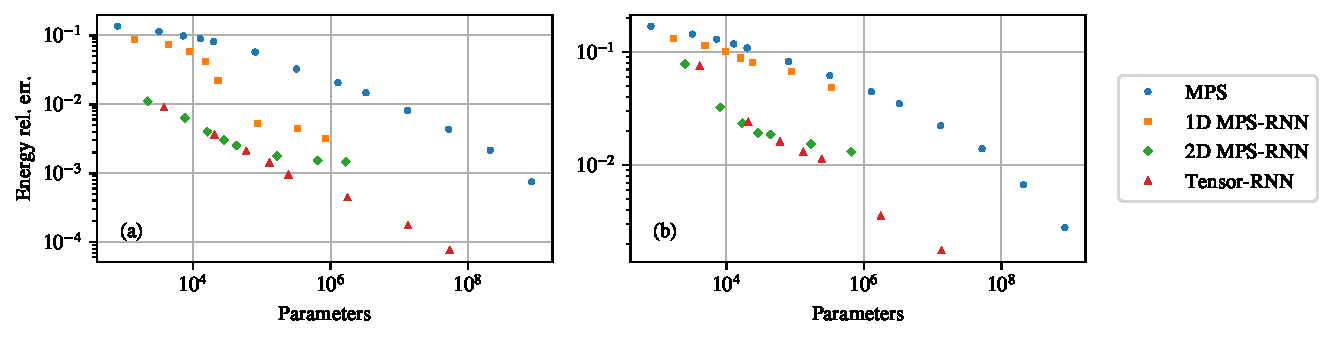
\includegraphics[width=1.1\linewidth]{ch9/tensor_rnn_energy_param.pdf}
\caption[Variational energy vs. number of parameters for tensor-RNN]{
Variational energy as a function of the number of parameters, in the same setting as \cref{fig:tensor-rnn-energy-chi}.
This figure is reproduced from Fig.~S3 in the supplemental material for Ref.~\cite{wu2023tensor}.
}
\label{fig:tensor-rnn-energy-param}
\end{figure}

The tensor-RNN has better parameter efficiency than the original MPS on both the square and the triangular lattices. However, we remark that the relative error on the triangular lattice is higher than that on the square lattice by an order of magnitude for all ansatzes in the plot, which means the frustrated sign structure is still a challenge for the tensor-RNN.

\subsection{Spatial correlations}
\label{sec:tensor-rnn-corr}

\begin{figure}[!b]
\centering
\hspace*{-0.05\linewidth}
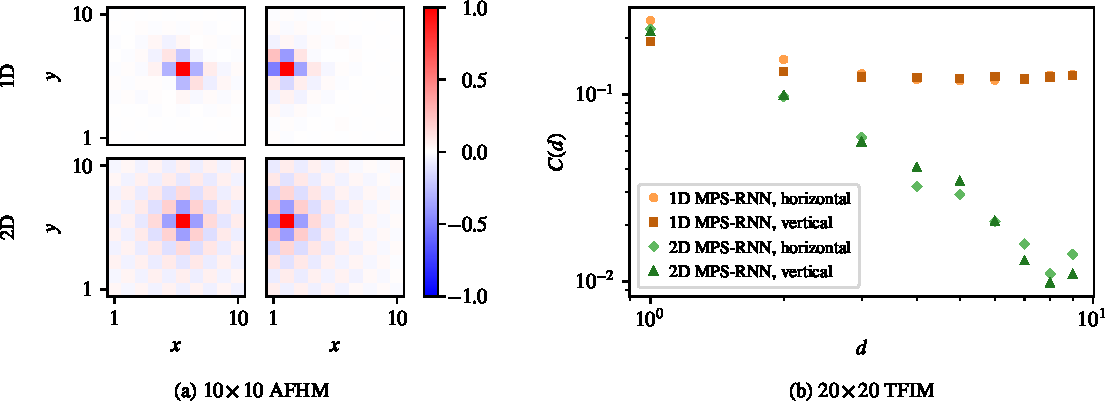
\includegraphics[width=1.05\linewidth]{ch9/tensor_rnn_corr.pdf}
\caption[Spin correlations in MPS-RNN]{
(a) Correlations of all spins $s_{x, y}$ with the spin $s_{5, 5}$ (left column) and $s_{1, 5}$ (right column) for the AFHM on the $10 \times 10$ square lattice with OBC, given by the 1D MPS-RNN (top row) and the 2D MPS-RNN (bottom row) with bond dimension $\chi = 10$. \\
(b) Correlation $C(d)$ as a function of the distance $d$ in \cref{eq:corr-d} for the TFIM at its critical point $\Gamma = 3$, on the $20 \times 20$ square lattice with OBC, in horizontal and vertical directions, given by the 1D MPS-RNN and the 2D MPS-RNN.
This figure is reproduced from Fig.~S4 in the supplemental material for Ref.~\cite{wu2023tensor}.
}
\label{fig:tensor-rnn-corr}
\end{figure}

Next, we examine the ability of our ansatzes to capture spatial correlations in 2D systems. A qualitative visualization of the correlations with a certain spin is shown in \cref{fig:tensor-rnn-corr}~(a) for the AFHM. The 2D MPS-RNN successfully produces isotropic and long-range correlations, as expected in \cref{sec:2d-mps-rnn}, while the 1D one fails to do so.

To demonstrate the particularly interesting case of algebraically decaying correlations in 2D critical systems, we use the TFIM at its critical point $\Gamma = 3$, and increase the lattice size to $20 \times 20$ to better investigate the asymptotic behavior. As shown in \cref{fig:tensor-rnn-corr}~(b), the 2D MPS-RNN correctly captures the algebraically decaying correlations in both horizontal and vertical directions, which can be fitted by a straight line on the log-log plot, while the 1D one can only produce constant correlations in the long range.

\subsection{Magnitudes of tensor, matrix, and vector terms}
\label{sec:tensor-rnn-magnitude}

\begin{figure}[htb]
\centering
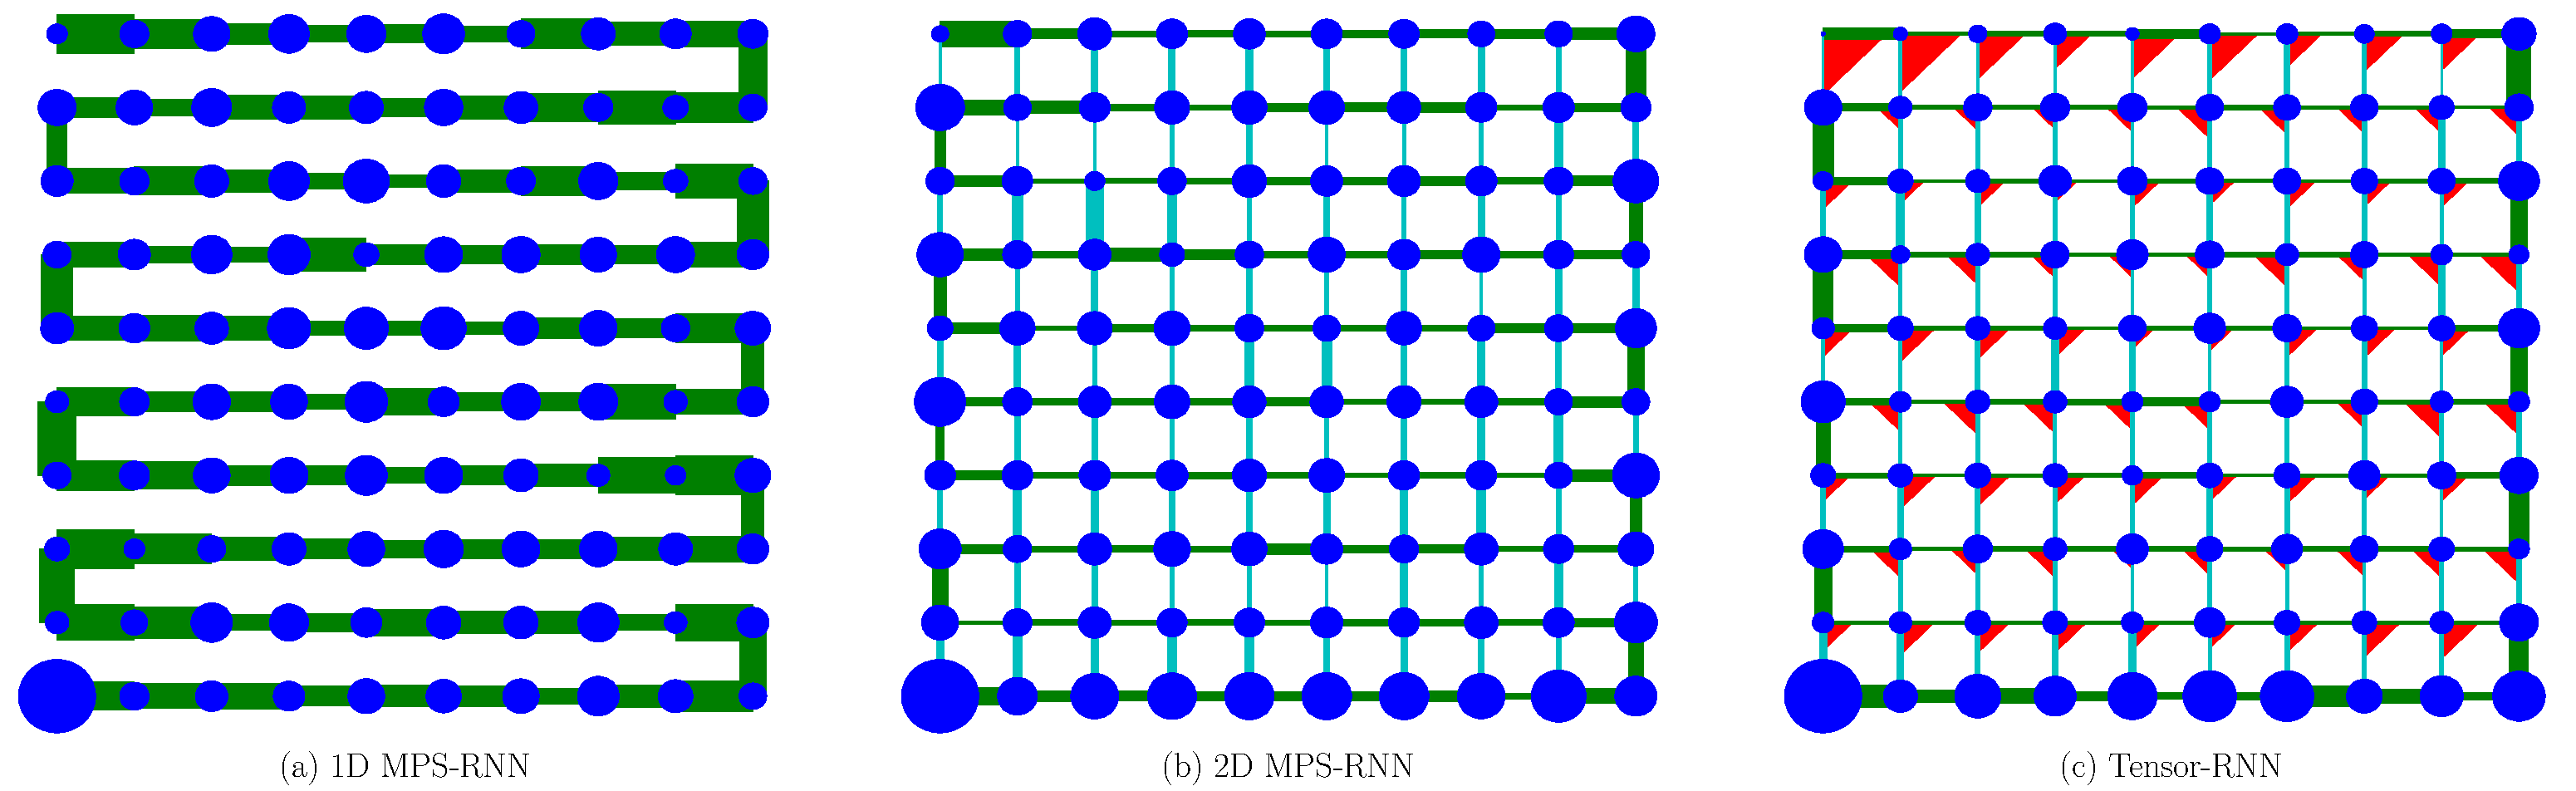
\includegraphics[width=\linewidth]{ch9/tensor_rnn_h_comp.pdf}
\caption[Contributions of tensor, matrix, and vector terms in tensor-RNN]{
Contributions of the tensor term $\tilde{T}^{(x, y)}$ (areas of {\color[HTML]{d62728} red} triangles), the matrix terms $\tilde{M}^{(x, y)}_\text{x}$, $\tilde{M}^{(x, y)}_\text{y}$ (areas of rectangles), and the vector term $\tilde{v}^{(x, y)}$ (areas of {\color[HTML]{1f77b4} blue} circles) to the memory $\vh^{(x, y)}$ at each site, in (a) 1D MPS-RNN, (b) 2D MPS-RNN, and (c) tensor-RNN with bond dimension $\chi = 10$, trained for the AFHM on the $10 \times 10$ square lattice with OBC.
In the matrix terms, the {\color[HTML]{2ca02c} green} rectangles are along the snake order, and the {\color[HTML]{9467bd} purple} ones are not.
This figure is reproduced from Fig.~S5 in the supplemental material for Ref.~\cite{wu2023tensor}.
}
\label{fig:tensor-rnn-h-comp}
\end{figure}

When evaluating the above ansatzes, the memory $\vh^{(x, y)}$ at each site can consist of contributions from the tensor terms, the matrix terms, and the vector term, and it is worth investigating their respective magnitudes. Considering how $\vh^{(x, y)}$ is used in \cref{eq:mps-rnn-p-eta} to compute the probability, we define the $2$-norms weighted by $\vet^{(x, y)}$:
\begin{align}
\norm{T}^{(x, y)}(\vs) &= \sqrt{\sum_a \eta^{(x, y)}_a \left| \sum_{b, c} T^{(x, y)}_{s_{x, y}; a, b, c} h^{(x - 1, y)}_b h^{(x, y - 1)}_c \right|^2}, \\
\norm{M}^{(x, y)}_\text{x}(\vs) &= \sqrt{\sum_a \eta^{(x, y)}_a \left| \sum_b M^{(x, y)}_{\text{x}; s_{x, y}; a, b} h^{(x - 1, y)}_b \right|^2}, \\
\norm{M}^{(x, y)}_\text{y}(\vs) &= \sqrt{\sum_a \eta^{(x, y)}_a \left| \sum_b M^{(x, y)}_{\text{y}; s_{x, y}; a, b} h^{(x, y - 1)}_b \right|^2}, \\
\norm{v}^{(x, y)}(\vs) &= \sqrt{\sum_a \eta^{(x, y)}_a \left| v^{(x, y)}_{s_{x, y}; b} \right|^2},
\end{align}
assuming $x$ increases in the snake order. As they are functions of the spin configuration $\vs$, we further define the averages
\begin{equation}
\overline{\norm{T}}^{(x, y)} = \sum_\vs q(\vs) \norm{T}^{(x, y)}(\vs),
\end{equation}
and similarly $\overline{\norm{M}}^{(x, y)}_\text{x}$, $\overline{\norm{M}}^{(x, y)}_\text{y}$, and $\overline{\norm{v}}^{(x, y)}$, which are all estimated by Monte Carlo sampling. To ease the visualization, we normalize them at each site:
\begin{equation}
\tilde{T}^{(x, y)} = \frac{\overline{\norm{T}}^{(x, y)}}{\overline{\norm{T}}^{(x, y)} + \overline{\norm{M}}^{(x, y)}_\text{x} + \overline{\norm{M}}^{(x, y)}_\text{y} + \overline{\norm{v}}^{(x, y)}},
\end{equation}
and similarly $\tilde{M}^{(x, y)}_\text{x}$, $\tilde{M}^{(x, y)}_\text{y}$, and $\tilde{v}^{(x, y)}$.

The results are visualized in \cref{fig:tensor-rnn-h-comp}. In the 1D MPS RNN, the matrix terms are particularly large near the ends of rows, because they need to transfer all information about the current row to the next row. While in the 2D MPS RNN, most matrix terms have the same order of magnitude regardless of their directions. In the tensor-RNN, the interesting phenomenon is that the tensor terms are particularly large only in the last row, which are essential to produce the area law of entanglement entropy, as expected in \cref{sec:tensor-rnn}. On the contrary, if there is a large tensor term on every site, then a volume law would be produced.

\section{Conclusion}

In conclusion, the tensor-RNN ansatz is a hybrid architecture between TN and RNN taking both advantages. Compared to MPS which can only produce $O(\ln \chi)$ entanglement entropy and exponentially decaying correlations, there are both analytical and numerical evidence for tensor-RNN to produce the 2D area law of entanglement entropy, as well as numerical evidence for the algebraically decaying correlations in 2D critical systems. Compared to PEPS which has exponentially high computational cost, tensor-RNN supports efficient evaluation in polynomial time, as well as exact sampling in the AR order. As a result, tensor-RNN has higher parameter efficiency than MPS, and also achieves better accuracy of variational approximation than PEPS in a practical computation time.

On the other hand, compared to conventional RNN architectures which are difficult to analytically study and adaptively scale up, the simple multilinear architecture of tensor-RNN allows us to investigate its analytical properties, and systematically improve its accuracy by increasing the bond dimension. The exact mapping from MPS to tensor-RNN leads to the hierarchical initialization, which makes it possible to optimize tensor-RNN with numerous parameters. It remains an open question to exactly construct more 2D states of interest using tensor-RNN, such as the RVB state and the toric code, or provide analytical evidence for the algebraically decaying correlations.
